\input{preamble}


\begin{document}
\begin{singlespace}
\title{Final Proposal}
\author{Austyn West\thanks{Department of Economics, Texas A\&M University.}}
\date{December 4, 2025}
\maketitle
\end{singlespace}

\section*{Introduction}

Human capital, widely recognized as a primary driver of economic growth and individual prosperity, is fundamentally shaped by educational attainment \citep{mincer1974, hanushek2012}. In the 21st century, the formation of human capital is increasingly mediated by digital technology, making reliable, high-speed internet access a critical input in the educational production function. Recognizing this, the U.S. government established the E-Rate program in 1996 to subsidize telecommunications and internet access for schools and libraries. For nearly two decades, the program provided basic connectivity. However, shift occurred in 2014 with the E-Rate Modernization Order, which fundamentally reconfigured the program to meet the demands of digital learning. The reform explicitly prioritized high-speed broadband infrastructure and, for the first time, provided dedicated funding for internal Wi-Fi networks, all while increasing the program's funding cap by over 60 percent.

This study estimates the causal effect of this major federal investment in educational technology on student attainment. We ask: Did the 2014 E-Rate modernization, by accelerating the deployment of high-speed broadband and Wi-Fi in public schools, improve academic performance, increase high school graduation and college enrollment, and enhance long-term earnings? Furthermore, did the reform's design, which targeted resources through a discount matrix based on poverty and location, successfully mitigate persistent disparities in the digital divide?

The existing literature provides a complex backdrop. A foundational body of work establishes the significant returns to educational investment \citep{mincer1974, hanushek2012} and the importance of school infrastructure for learning \citep{berner1993, park2020}. Research specifically on technology, however, offers mixed evidence. Early studies on school computing often found limited effects on standardized test scores \citep{angrist2002, beuermann2013}, and initial evaluations of basic broadband connectivity similarly showed muted impacts \citep{hazlett2019}. More recent research suggests that the quality of connectivity, measured by speed, may be a more potent factor, with some estimates indicating that improvements in broadband speed can boost test scores by magnitudes comparable to other successful educational interventions \citep{sanchis2021, duflo2012}. Concurrently, a separate strand of literature meticulously documents the stubborn persistence of the digital divide, with significant gaps in broadband access and quality along racial, income, and geographic lines \citep{gallardo2024, li2023, reddick2020}. What remains less clear is whether large-scale, targeted public policy can effectively overcome these barriers and translate enhanced digital infrastructure into meaningful gains in human capital development.

We contribute to this literature by providing the first causal evaluation of the 2014 E-Rate modernization's impact on a comprehensive set of educational outcomes. Leveraging rich administrative data from Texas public schools and detailed E-Rate funding records, we employ a Difference-in-Discontinuities (DiDisc) design \citep{grembi2016}. This empirical strategy exploits the sharp discontinuities in E-Rate subsidy rates at specific poverty thresholds both before and after the 2014 reform. By comparing the change in outcomes for schools just above and just below these eligibility cutoffs, we isolate the local average treatment effect of the policy change.

This paper will demonstrate whether public investment in educational technology can yield substantial returns. The 2014 E-Rate modernization, by shifting focus from basic connectivity to high-speed broadband and robust internal networks, played a pivotal role in enhancing human capital formation for a generation of students. The results underscore the importance of both the quantity and quality of digital infrastructure and offer timely insights for policymakers considering future investments in the nation's educational and technological foundation.

\section*{Literature Review}

The literature on broadband infrastructure and educational outcomes is broad and interdisciplinary, spanning work in education economics, public finance, and information technology policy. Three areas are particularly relevant to the 2014 E-Rate modernization: (i) the effects of digital access and technology adoption on human capital formation, (ii) the role of infrastructure investments in school environments and learning outcomes, and (iii) the persistence of the digital divide and heterogeneity in broadband access.

\textbf{Technology, Connectivity, and Human Capital Formation.} The role of education in human capital formation is a cornerstone of economic theory. \citet{mincer1974} established the Mincer equation, showing that each additional year of schooling increases individual earnings by roughly 5–8\%, demonstrating the microeconomic returns to education. \citet{hanushek2012} provide complementary macro-level evidence, finding that improvements in cognitive skills are associated with a 2 percentage point higher annual GDP growth rate across nations over 40 years. Closely related broadband research, such as \citet{hazlett2019}, indicates that basic connectivity alone had limited effects on standardized test scores, suggesting that technology must be effectively integrated to impact human capital. Together, these studies highlight both the magnitude of returns to education and the potential, but conditional, role of digital infrastructure in enhancing learning outcomes.

\textit{Broadband Access.}  Research shows that broadband availability can shape educational opportunities through development of skills and enhanced learning activities. Studies such as \citet{hazlett2019}, \citet{dettling2015}, and \citet{niewoehner2025} suggest that connectivity influences learning environments, though limited improvements in SAT scores prior to 2014 \citep{hazlett2019} highlight the constraints of basic access. Earlier work by \citet{angrist2002}, \citet{angrist2009}, \citet{beuermann2013}, and \citet{duflo2012} highlights how interventions targeting teachers can improve student outcomes. For example, \citet{duflo2012} show that increasing teacher attendance through incentive programs raised student test scores by 0.17 standard deviations after one year. While Duflo et al. focus on direct incentives, these findings conceptually illustrate that enhancing teacher effectiveness can boost student human capital. In the context of broadband, providing teachers with reliable high-speed internet and digital tools may similarly increase their capacity to deliver high-quality instruction, thereby amplifying student learning outcomes.

\textit{Broadband Speed.} The quality of broadband, measured by speed, also affects educational delivery. Studies examining broadband quality show that higher-speed connections facilitate advanced learning tools. \citet{sanchis2021} report that a one-standard deviation increase in broadband speed raises test scores by 0.19 standard deviations, comparable in magnitude to teacher incentive effects from \citet{duflo2012}. \citet{boeri2023} and \citet{grimes2018} further emphasize that the effectiveness of broadband depends on socioeconomic and infrastructural conditions, indicating that speed alone is insufficient to uniformly enhance educational outcomes.

The pre-reform focus on connectivity \citep{hazlett2019} and the limited post-reform evaluation leave a significant gap in understanding the dynamic relationship between broadband technologies and human capital development across diverse socioeconomic and geographic contexts. This study addresses this gap by estimating the causal impact of the 2014 E-Rate modernization on graduation rates, college enrollment, and earnings, investigating how enhanced access and speed collectively reshape human capital formation. 

\textbf{Infrastructure Investments in School Environments and Learning Outcomes.}  The influence of school infrastructure on educational outcomes has long been a focus of empirical research. Early studies by \citet{berner1993}, \citet{cash1993}, and \citet{duran2008} establish that physical conditions, such as building quality and classroom environment, play a pivotal role in student performance and attendance with \citet{berner1993} finding a positive association between building condition improvements and student achievement.  Subsequent work by \citet{maxwell1999}, \citet{hathaway1995}, and \citet{park2020} extends this to environmental factors like lighting and temperature. A study by \citet{park2020} finds that without air conditioning, a one degree hotter school year reduces that year’s learning by one percent. More recently, \citet{wanke2024} and \citet{daoud2021} emphasize the growing importance of technological infrastructure, including broadband and home internet, as mediators of educational success, with \citet{wanke2024} explaining 30–40\% of performance variance through infrastructure and teacher capital. Together, these studies suggest that investments in both physical and technological assets can enhance educational quality through giving students access to quality broadband infrastructure and potentially increasing the human capital of teachers.

This study contributes by evaluating how the 2014 E-Rate modernization’s focus on broadband and Wi-Fi infrastructure impacts attainment outcomes, building on existing infrastructure research to examine the impact of broadband infrastructure and quality on educational outcomes.

\textbf{The Digital Divide and Heterogeneity in Broadband Access.}  Disparities in broadband access and quality across geographic and demographic lines persist. \citet{gallardo2022} and \citet{gallardo2024} highlights continuing rural–urban and socioeconomic gaps, with \citet{gallardo2024} noting that as the share of the rural population, the population age 65 or older, and individual poverty rates increased, the average download speed decreased. Whereas, \citet{li2023} and \citet{reddick2020} identify racial and income-based disparities often tied to affordability and infrastructure deficits, with \citet{li2023} finding that broadband access in majority Black and Hispanic neighborhoods was 10–15\% lower than in majority White or Asian neighborhoods. \citet{reddick2020} shows that lower-income and minority groups are more likely to have basic connectivity but rarely benefit from high-speed options due to affordability barriers. Historical studies (\citet{strover2001}, \citet{riddlesden2014},  \citet{kelley2020}) trace the evolution of these disparities in the U.S. and internationally. \citet{boeri2023} further notes that wealthier communities disproportionately access higher-speed broadband. 

This study advances the literature by analyzing how the 2014 E-Rate reforms mitigate digital disparities and contribute to attainment gains, particularly in underserved regions, aligning with the proposal’s emphasis on equity and rural development.


\section*{Data}

\textbf{Data Sources.} This study combines two primary administrative datasets. The first is the Texas Academic Performance Reports (TAPR), published annually by the Texas Education Agency (TEA), which provides school-level data on student performance, demographics, and college readiness from the 2012–13 through 2018–19 school years. The second is the federal E-Rate program data, which contains school-level records on requested and approved funding for telecommunications and internet services.\footnote{The E-Rate data are provided by the Universal Service Administrative Company (USAC) and consist of Service Provider Invoice Forms (Form 472) and Billed Entity Applicant Reimbursement Forms (Form 474).}

\textbf{E-Rate Funding Structure.} The E-Rate program provides subsidies for two categories of services. Category One covers broadband internet access to the school, while Category Two covers internal connections, primarily Wi-Fi networks and related equipment within schools. Discount levels are determined by the percentage of students in a district eligible for the National School Lunch Program (NSLP), a standard measure of economic disadvantage. This creates sharp eligibility thresholds at 1\%, 20\%, 35\%, 50\%, and 75\% NSLP eligibility. For example, districts with at least 75\% of students eligible for NSLP receive the maximum discount of up to 90\%.

\textbf{Sample Construction.} The unit of analysis is the school-year. The sample includes all Texas public schools that appear in TAPR for every year from 2012–13 through 2018–19. To ensure data consistency and comparability, we apply two key restrictions. First, we exclude small "1A" schools (those with fewer than 105 students) due to frequent data suppression for small subgroups. Second, we exclude juvenile justice, disciplinary alternative, and charter schools with non-standard testing and grading structures.

\textbf{Key Outcome Variables.} Our analysis examines a range of academic outcomes. For elementary and middle schools, we use results from the State of Texas Assessments of Academic Readiness (STAAR). We focus on the rate of students Requiring Accelerated Instruction, a consistent metric across our sample period that captures the proportion of students failing to meet the passing standard.\footnote{This measure is part of the Student Success Initiative (SSI). While reporting labels changed, the underlying failure rate seems consistent.} For high schools, we analyze graduation rates, dropout rates, SAT/ACT participation and performance, and broader college readiness metrics.

\textbf{Data Limitations.} Several data issues require careful consideration. First, changes in the TEA's reporting of STAAR outcomes over time necessitate the construction of consistent measures. Second, the E-Rate data reflect approved funding, which may not perfectly align with the timing of service implementation due to lags between application, approval, and installation.\footnote{The data also do not include applications that were denied or were still pending, which limits the analysis of overall demand.} Finally, some subgroup data remain partially masked even in larger schools, requiring robust handling of missing values.

\section*{Descriptive Statistics}


Table~\ref{tab:erate_summary_stats} presents summary statistics for E-Rate funding requests submitted by Texas public school districts. Panel A reports continuous financial measures, including requested amounts, approved amounts, and discount rates, while Panel B summarizes binary indicators of application status.

The distribution of requested amounts exhibits substantial right-skewness. The mean request is \$11,902, but the 75th percentile is only \$4,580, indicating that the mean is heavily influenced by a small number of large requests. This skewness motivates the use of logarithmic transformations in subsequent analyses, where the log requested amount has a more symmetric distribution with mean 7.31 (SD 2.08). The substantial right-skewness of the requested amounts is visually confirmed in Figure~\ref{fig:log_density}, which plots the density of the natural logarithm of requested amounts. While the raw dollar amounts are heavily skewed, the log-transformed variable approximates a symmetric, bell-shaped distribution, validating the use of logarithmic transformations in our multivariate analyses.

Approved amounts follow a similar pattern, with mean \$10,081 (SD \$74,060), suggesting modest adjustments during the review process. The discount rate distribution shows meaningful variation across districts, ranging from 60\% at the 25th percentile to 85\% at the 75th percentile around a mean of 70.6\%, reflecting the program's design where discounts are tied to the percentage of students eligible for the National School Lunch Program.

Panel B reveals that most funding requests are successful, with 91.8\% receiving at least partial approval. Only 0.3\% of requests have nonpositive amounts, suggesting high data quality. The reimbursement flag (9.7\%) and funded with comment flag (1.7\%) indicate that while most applications are processed routinely, a nontrivial minority require additional administrative review.

\begin{table}[htbp]
\centering
\caption{Summary Statistics for E-Rate Funding Requests}
\label{tab:erate_summary_stats}
\begin{threeparttable}
\begin{tabular}{ l c c c c }
\toprule
& \textbf{Mean} & \textbf{Std. Dev.} & \textbf{25th pct.} & \textbf{75th pct.} \\
& (1) & (2) & (3) & (4) \\
\midrule
\multicolumn{5}{l}{\underline{\textbf{Panel a. Financial Amounts}}} \\ \\
\hspace{2mm} \textbf{\textit{Requested Invoice Amount}} & 11,902 & 90,203 & 480 & 4,580 \\
\hspace{2mm} \textbf{\textit{Approved Invoice Amount}} & 10,081 & 74,060 & 275.230 & 3,868 \\
\hspace{2mm} \textbf{\textit{Log Requested Amount}} & 7.310 & 2.083 & 6.186 & 8.431 \\
\hspace{2mm} \textbf{\textit{Discount Rate}} & 70.644 & 20.355 & 60 & 85 \\ \\
\\ \\
\multicolumn{5}{l}{\underline{\textbf{Panel b. Flags and Status}}} \\
\hspace{2mm} \textbf{\textit{Funded Flag}} & 0.918 & 0.274 & & \\
\hspace{2mm} \textbf{\textit{Negative Requested Amount Flag}} & 0.003 & 0.056 & & \\
\hspace{2mm} \textbf{\textit{Reimbursement Flag}} & 0.097 & 0.295 & & \\
\hspace{2mm} \textbf{\textit{Funded with Comment}} & 0.017 & 0.128 & & \\
\bottomrule
\end{tabular}
\footnotesize
\textit{Notes:} This table reports summary statistics for E-Rate funding requests submitted by public school districts in Texas. Amount Requested refers to the total pre-discount funding amount submitted on Form 471. Approved Amount is the total amount approved for reimbursement. Log Total Amount is the natural logarithm of the requested amount after removing zero or negative values. Discount Rate is the applicant's E-Rate discount percentage based on the percentage of students on the National School Lunch Program in the district. Binary indicator variables are defined as follows: Funded Flag equals 1 if any portion of the request was approved; Negative Amount Flag equals 1 for filings with nonpositive or invalid pre-discount amounts; Reimbursement Flag equals 1 if the request includes a reimbursement decision code; and Funded with Comment equals 1 for requests that were both funded and accompanied by a reimbursement decision code. Percentile columns reflect the empirical 25th and 75th percentiles of each distribution.
\end{threeparttable}
\end{table}


\begin{figure}[h!]
    \centering
    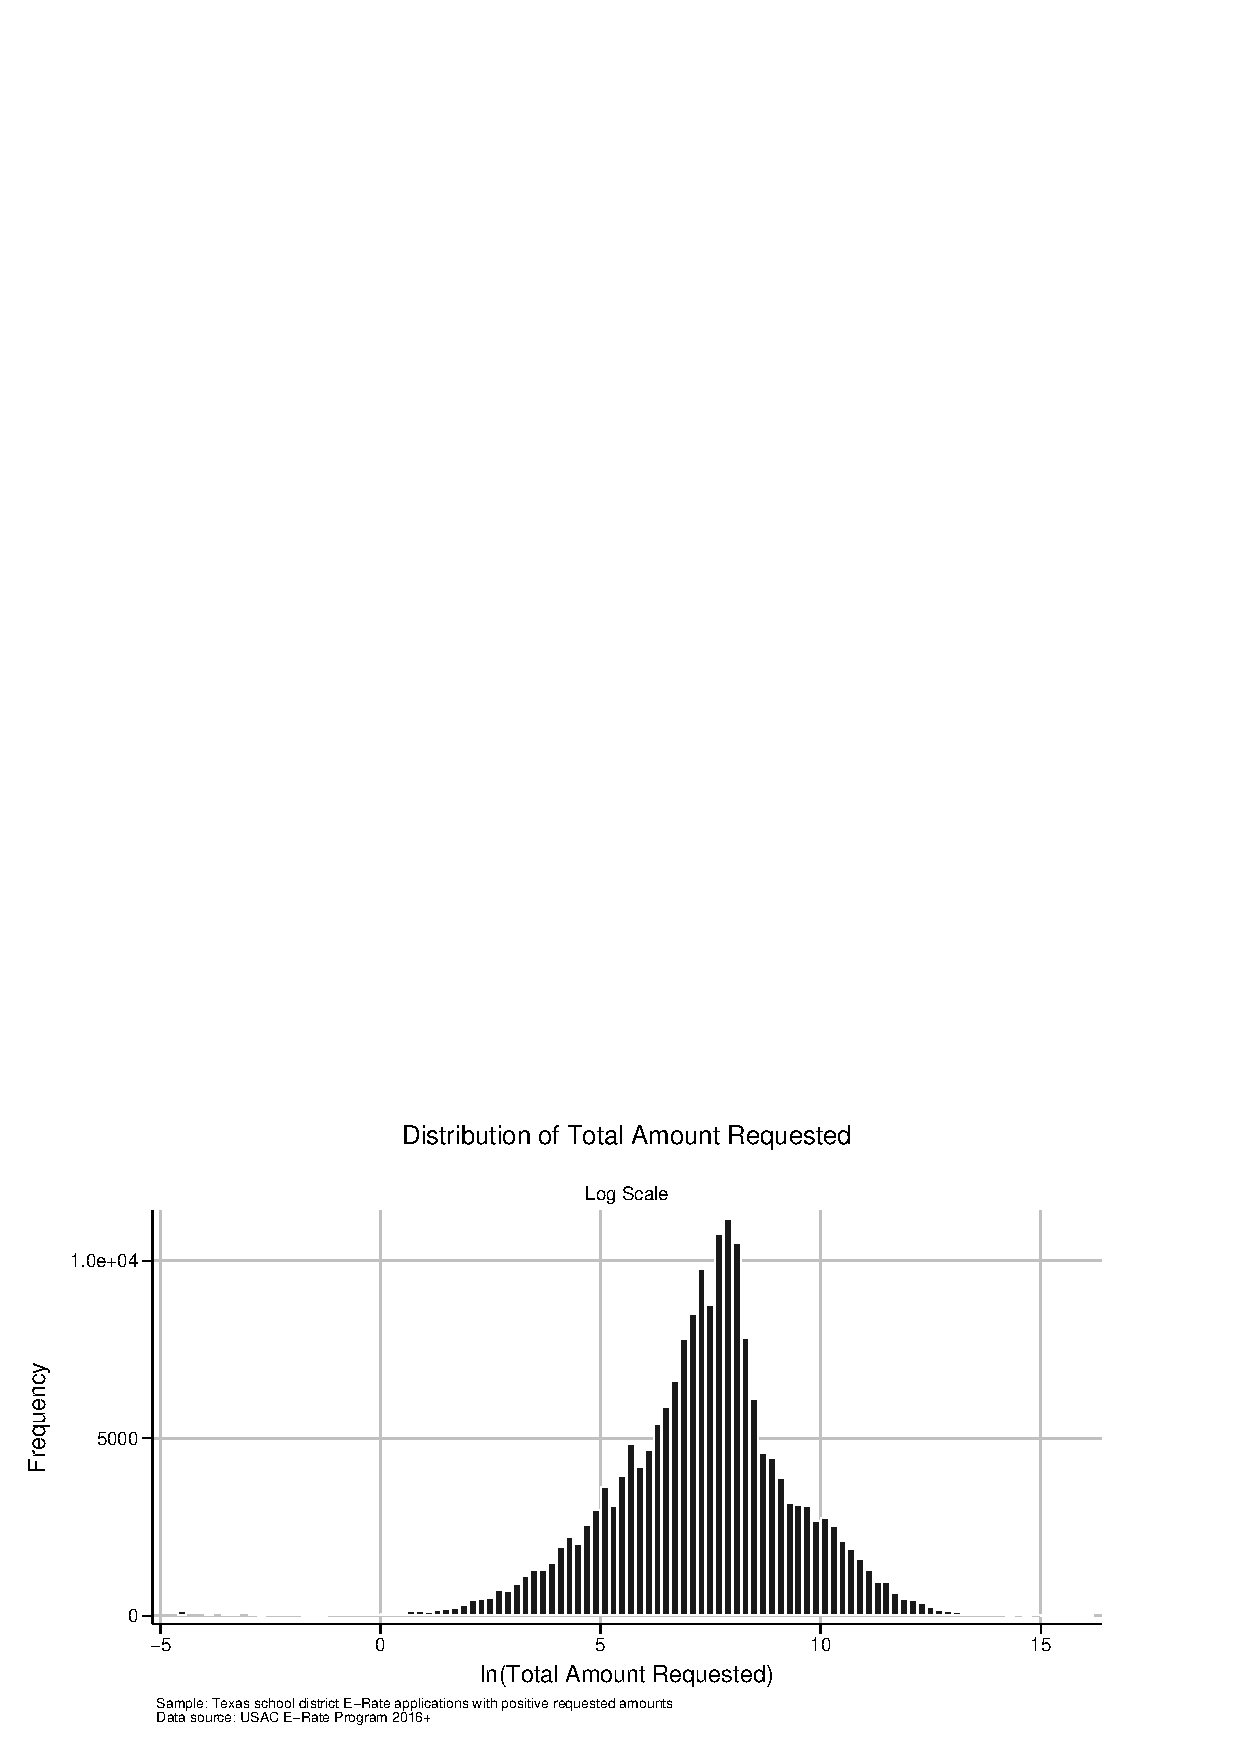
\includegraphics[width=0.8\linewidth]{Log_Amount_Requested_Density.pdf}
    \caption{Distribution of the Log-Transformed Total Amount Requested}
    \label{fig:log_density}
    \begin{minipage}{0.8\linewidth}
        \footnotesize
        \textit{Note:} This figure displays the frequency distribution of the natural logarithm of total funding amounts requested by Texas school districts in their E-Rate applications. The distribution is approximately normal, centered around a log value of 5-10, with a positive skew indicating a minority of applications requested substantially larger amounts. The log transformation reveals the underlying shape of the data, which would be heavily right-skewed in its original dollar-scale form.
    \end{minipage}
\end{figure}


These summary statistics reflect the underlying economics and administration of the E-Rate program. The heavy-tailed distribution of requested amounts likely stems from the large fixed costs associated with network infrastructure, which generates a few very large requests from districts undertaking major upgrades, alongside many smaller requests for recurring services. The high approval rate is consistent with the program's goal of universal service support, where applications are pre-screened for eligibility.

These patterns have several implications for our empirical strategy. The heavy-tailed distribution of financial amounts suggests that median regressions or models using logarithmic transformations may be more appropriate than linear models using levels. The systematic variation in discount rates, which is quasi-exogenous as it is tied to a district's socioeconomic profile, provides the source of identifying variation for our Difference-in-Discontinuities design. The descriptive evidence thus supports modeling approaches that account for the program's institutional features and the distributional characteristics of the key variables.

\section*{Empirical Design}

This study applies a Difference-in-Discontinuities (DiDisc) framework developed by \citet{grembi2016} to identify the causal effect of the 2014 E-Rate Modernization Order on educational outcomes in Texas public schools. The DiDisc approach combines a regression discontinuity (RD) in program eligibility with a time discontinuity at the start of the policy reform. By differencing out any pre-existing jump in outcomes at each eligibility threshold, the design isolates the reform-induced change in the discontinuity and can therefore identify the local causal effect of the 2014 policy change.

\textbf{Institutional Background.} The 2014 reform substantially altered the structure of E-Rate funding. It raised the annual cap from \$2.4 billion to \$3.9 billion, prioritized high-speed broadband (Category 1) connections, and introduced per-student budgets for internal Wi-Fi (Category 2) services. The maximum subsidy rate for Category 2 was reduced from 90 percent to 85 percent. E-Rate discounts are determined at the district level according to the share of students eligible for the National School Lunch Program (NSLP), generating a series of discrete jumps in funding generosity at eligibility thresholds. Major thresholds occur at 1, 20, 35, 50, and 75 percent NSLP.\footnote{See Universal Service Administrative Company, ``E-Rate Discount Matrix,'' \url{https://www.usac.org/wp-content/uploads/e-rate/documents/samples/Discount-Matrix.pdf}.} For example, districts with between 75 and 100 percent of students eligible for NSLP qualify for the maximum 90 percent and 85 percent discounts on Category 1 and Category 2 services, respectively. Urban and rural distinctions slightly affect the precise discount levels, but the key forcing variable is the NSLP percentage.

\textbf{Identification Strategy.} The design uses both the discontinuous variation in E-Rate discount rates at these NSLP thresholds and the time variation induced by the 2014 reform. This dual source of variation enables estimation of local causal effects for schools near each eligibility boundary. The baseline analysis centers on the 75 percent threshold, where the reform most likely produced the largest change in funding intensity, while additional analyses examine the 20, 35, and 50 percent cutoffs to assess robustness and potential heterogeneity in treatment effects across the discount matrix. For each cutoff $c$, the specification takes the form
\begin{align}
Y_{ist}
&= \beta_{0c} + \beta_{1c}\text{Post}_t + \beta_{2c}\text{Above}_{ic} + \beta_{3c}(\text{Post}_t \times \text{Above}_{ic}) \nonumber \\
&\quad + f_c(X_{it}) + f_c(X_{it}) \cdot \text{Post}_t + f_c(X{it}) \cdot \text{Above}_{ic} \nonumber \\
&\quad + \mu_s + \tau_t + \varepsilon_{ist}.
\label{eq:didisc}
\end{align}

\textbf{Variable Definitions.} Here, $Y_{ist}$ denotes the outcome of interest such as the share of students meeting grade-level standards, SAT/ACT participation, dropout rates, or college readiness for school $s$ in district $i$ and year $t$. The first modernized funding year began disbursements in July 2015, corresponding to the 2015--16 school year; thus, $\text{Post}t=1$ for 2015--16 onward, reflecting the first full academic year after the reform. Pre-reform years provide three years of pre-trends. The running variable $X{it}$ measures the normalized distance of a district’s NSLP percentage from cutoff $c$. The function $f_c(X_{it})$ flexibly captures local trends around each threshold using local linear or low-order polynomial functions. School fixed effects $\mu_s$ control for time-invariant heterogeneity, and year fixed effects $\tau_t$ absorb common shocks. The coefficient $\beta_{3c}$ measures the Difference-in-Discontinuities estimate at cutoff $c$, representing the change in the outcome discontinuity at that threshold between the pre- and post-reform periods.

\textbf{Estimation.} The parameters of equation (\ref{eq:didisc}) are estimated using local linear regressions on either side of each cutoff within an optimal bandwidth, following \citet{calonico2014}. Robustness checks vary bandwidths and polynomial orders and compare results across thresholds to examine consistency of the reform’s effects along the NSLP distribution. Standard errors are clustered at the district level. The design allows for separate pre- and post-reform functional forms and distinct slopes on each side of the threshold, ensuring flexibility in the local fit and mitigating bias from misspecification.

\textbf{Identification Assumptions and Validation.} The key identifying assumption is that, in the absence of the reform, the difference in outcomes between districts just above and just below an NSLP eligibility threshold would have remained stable over time. This requires both continuity of potential outcomes across each threshold and local parallel trends in outcomes for districts near the cutoff. The primary threat to identification is strategic manipulation of the running variable by districts. We will test for this using density tests \citep{mccrary2008} and covariate balance checks across the cutoff in the pre-period. A further threat would be the occurrence of another contemporaneous policy or shock that differentially affected districts above versus below the NSLP thresholds. We will assess the validity of our identifying assumptions through several diagnostic tests. These include placebo tests using false reform years to confirm no effect is detected when none is expected, falsification exercises testing for spurious discontinuities at non-policy NSLP values, and formal pre-trend analyses to verify parallel outcomes in the pre-reform period. Evidence supporting these conditions would strengthen the causal interpretation of a significant $\beta_{3c}$ coefficient as the effect of the E-Rate modernization.


\section*{Conclusion}

This research proposes a rigorous evaluation of the 2014 E-Rate modernization's impact on educational outcomes in Texas. By leveraging a Difference-in-Discontinuities design that exploits sharp changes in funding generosity at specific poverty thresholds, the study aims to provide credible causal evidence on how investments in school broadband infrastructure affect human capital formation.

The project makes two primary contributions. First, it addresses a significant gap in the literature by providing the first causal evidence on the educational impacts of a major federal broadband infrastructure policy. While previous research has established correlations between technology and outcomes, this study's quasi-experimental design can isolate the causal effect of enhanced connectivity. Second, the analysis will shed light on whether the policy successfully mitigated educational disparities, with particular focus on heterogeneity by socioeconomic status and geographic location.

The feasibility of this research is supported by the availability of high-quality administrative data from both the E-Rate program and Texas education authorities. The clear, rule-based assignment of treatment through the NSLP discount matrix provides a strong foundation for identification. While challenges remain in data harmonization and model implementation, the research design is well-suited to address the central question of how broadband infrastructure investments translate into educational attainment. The findings will provide valuable evidence for policymakers considering future investments in educational technology and infrastructure, particularly as digital access becomes increasingly central to educational equity.

\newpage
\bibliographystyle{chicago}
\bibliography{Bibliography}

\end{document}